\section{The Bach4Popper Framework}
In this section, we introduce the methodology behind Bach4Popper,. 
We first present the overall system architecture. We then formalize its problem. 


\subsection{Problem Setting}
We now describe our problem setting. We consider a federated learning scenario with a set of $K$ clients $\mathcal{C} = \{C_1, \ldots C_n\}$. 
Each client $C_i$ hold a local dataset in the form of logic programs: $ D_i = (E_i^+,E_i^-, B_i)$ where $E_i^+$ and $E_i^-$ are respectively the sets of positive and negative examples respectively, and $B_i$ denotes local background knowledge expressed as logic programs. %This information remains strictly local and is never communicated to any other participant.
All clients share a common predicate declaration bias $\mathcal{D}$ that defines the structure of admissible hypotheses (e.g., target predicate, allowed body predicates, type and mode constraints). A central server $S$ coordinates hypothesis refinement, but has \textbf{no access} to any client’s data or background knowledge. This setup is formalized through the following components:
\begin{itemize}
    \item \textbf{Tester (Clients)} locally evaluate the current hypothesis $H_t$
    and produce outcomes $(\varepsilon_i^+, \varepsilon_i^-)$.
    \item \textbf{ $\mathcal{A}$ Aggregator (Server)} retrieves outcomes from the store and  combines them into a global result $(\varepsilon_g^+, \varepsilon_g^-)$.
    \item \textbf{Constrainer + Generator (Server)}, derive global symbolic constraints and generate refined hypotheses, following Popper’s generate–test–constrain methodology.
    \item $\mathcal{B}$ a communication layer ensuring decentralized interaction via Bach primitives (e.g., tell, ask, get).
\end{itemize}



\subsection{System Architecture}
Figure~\ref{fig:bachpopper} presents the overall architecture of our BACH4Popper framework. FedPopper decomposes Popper’s standard generate–test–constrain loop across the federation. The Server maintains the symbolic search state (hypothesis $H$, constraints) and is responsible for aggregating distributed outcomes, deriving global constraints, and
generating new candidate rules. As shown in the figure, clients hold private examples $(E_i^+, E_i^-, B_i)$ and act as Testers. They never reveal their data: instead, each client evaluates $H$ locally and produces $(\varepsilon_i^+, \varepsilon_i^-)$, indicating whether $H$ succeeds/fails to entail their examples. The BACH Store acts as a coordination medium. Components interact through ask/tell/get primitives:
\begin{itemize}
\item the server \emph{\textbf{tells}} the current hypothesis $H$;
\item clients \emph{\textbf{ask}} for $H$ to test it;
\item clients \emph{\textbf{tell}} outcome atoms $(\varepsilon_i^+, \varepsilon_i^-)$;
\item the server \emph{\textbf{gets}} all outcomes to refine the search.
\end{itemize}

This cycle repeats until the server receives the global outcome
$(\texttt{ALL}, \texttt{NONE})$, meaning that all positives are entailed and all negatives rejected. At that point, the final hypothesis has been collaboratively validated across all sites.
\begin{figure}
    \centering
    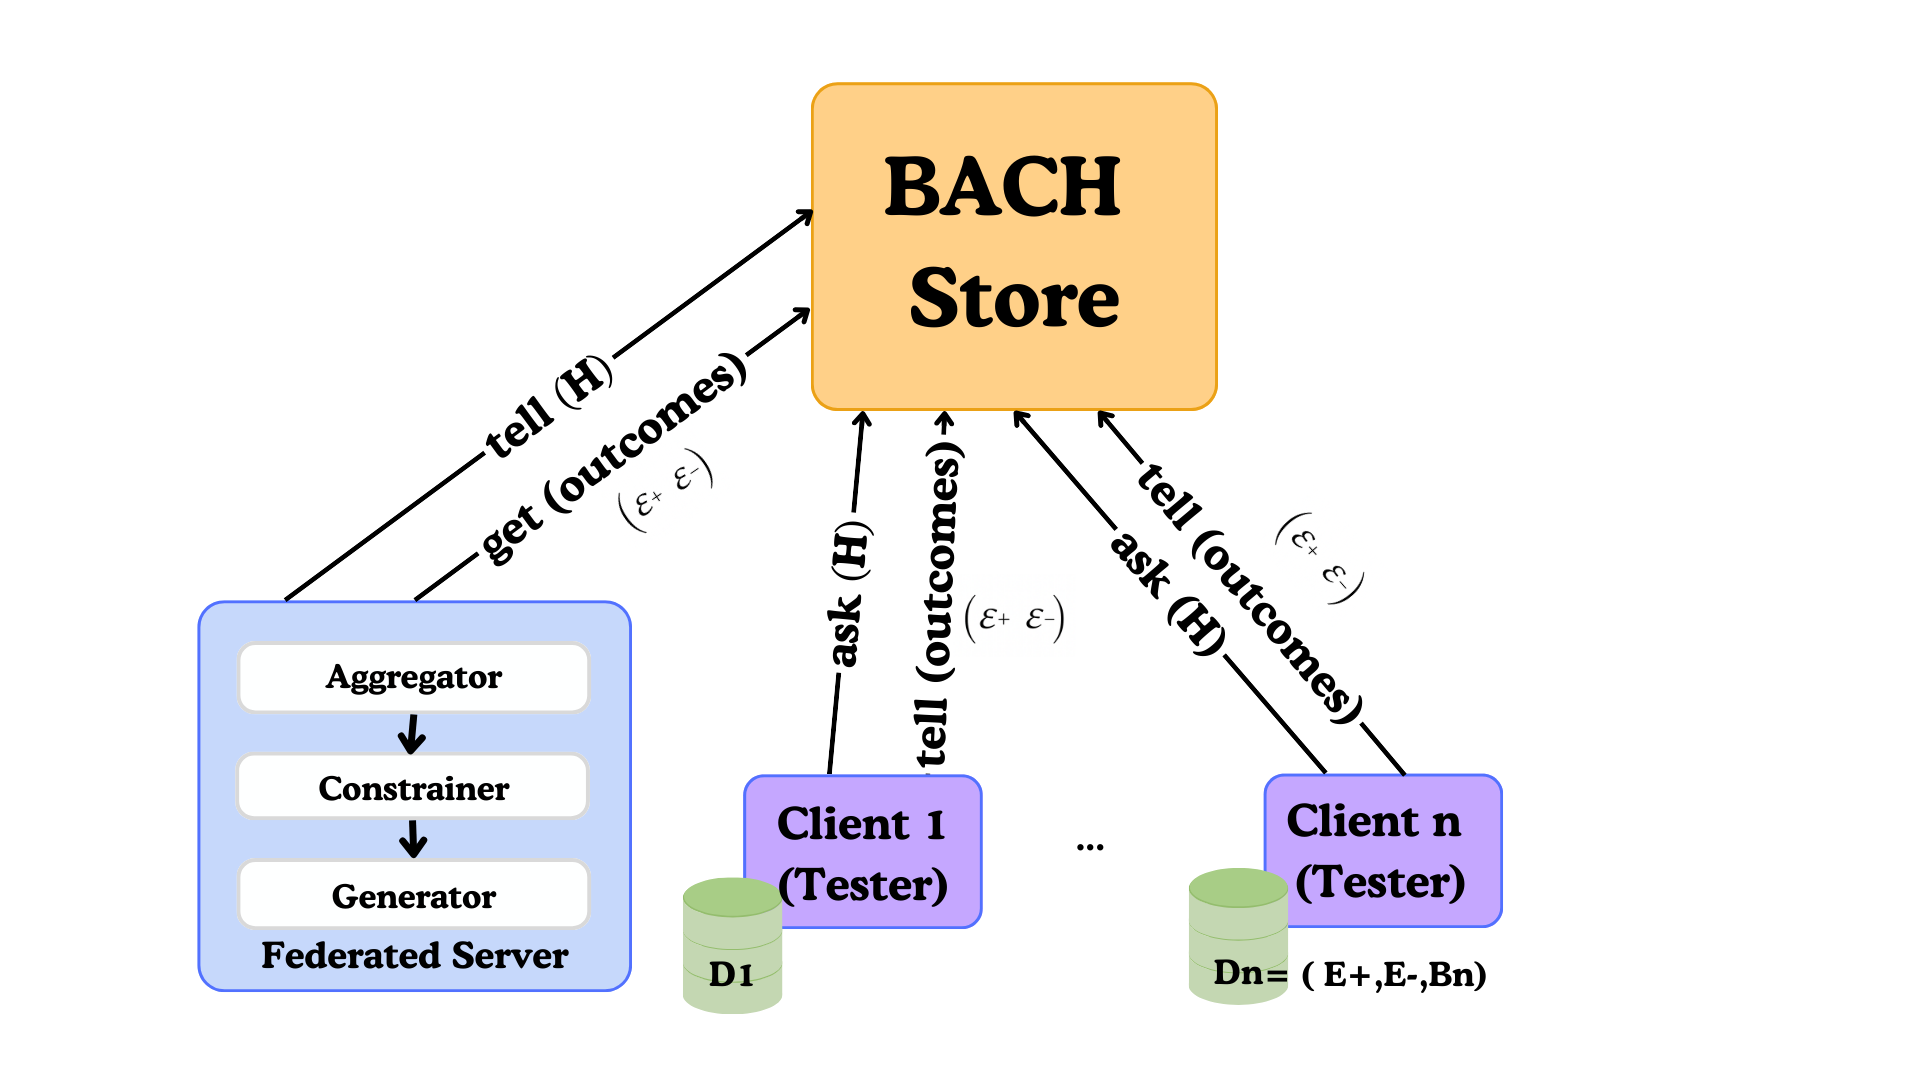
\includegraphics[width=\linewidth]{bach-popper.png}
    \caption{BACH4Popper Architecture}
    \label{fig:bachpopper}
\end{figure}


\subsection{Algorithm}

BACH4Popper (Algorithm~\ref{alg:bach4popper}) follows a structured orchestration between a shared coordination space or store (BACH), the federated server, and the distributed clients. The BACH store is started first to provide a shared medium for coordination messages (line 2).
Then, the server starts and initializes the first (possibly empty) hypothesis $H_0$ based on the provided predicate declarations (lines 6,7). This initial hypothesis is shared with the federation via a \textbf{\emph{tell($H_0$}} operation to BACH (line 8). Each client operates independently and in parallel (line 9). Clients retrieve the current hypothesis from the BACH store using an \textbf{\emph{ask(H)}} request (line 10), evaluates it locally on its private dataset using Popper’s \textbf{Test} procedure (line 11), and publishes the outcome back to BACH (line 12). Outcomes remain symbolic, only coverage failures are communicated, never raw data. The federated loop is driven entirely by these interactions.
At each round, the server gathers the outcomes reported by all clients (line 15) using the \textbf{\emph{get($\varepsilon_i^+, \varepsilon_i^- \})$)}} , and uses our implemented aggregatation function to aggregate a global coverage outcome  $(\varepsilon^+_g, \varepsilon^-_g)$ (line 16).
If this aggregated feedback indicates that the current hypothesis entails all positive examples and rejects all negative ones, i.e., 
$(\varepsilon^+_g,\varepsilon^-_g)= (ALL, NONE)$, the learning terminates successfully and the hypothesis returned (lines 17–18) is guaranteed to be globally correct.

Otherwise, the aggregated failures are used to build global constraints $C_t$ (line 20), which prune incorrect regions of the hypothesis space.
A refined hypothesis is then generated using Popper’s symbolic Generate step (line 21), and communicated back to all clients through another \textbf{\emph{tell}} to BACH (line 22).
This iterative refinement continues until convergence or until the maximum number of allowed rounds is reached.


\begin{algorithm}[ht]
\caption{\textsc{\textbf{Bach4Popper}}}
\label{alg:bach4popper}
\begin{algorithmic}[1]

\STATE \textbf{Launch Order:}
\STATE ~~(1) Start \textbf{BACH Store}  \hfill // Shared coordination space
\STATE ~~(2) Start \textbf{Server}
\STATE ~~(3) Start Clients $1 \dots K$ (Testers)

\vspace{4pt}
\STATE \textbf{Server Executes:}
\STATE ~~load predicate declarations $\mathcal{D}$
\STATE ~~Initialize $\mathcal{C}_t \;\text{with}\; \mathcal{D}$ 

\STATE ~~initialize first hypothesis $H_0$
\STATE ~~\textsc{\textbf{tell}}$(H_0)$ to BACH

\FOR{each round $t = 1,2,\ldots$}
\vspace{3pt}
    \FOR{each client $i$ in parallel}
    \STATE $(\varepsilon_i^+, \varepsilon_i^-)
                \leftarrow \textsc{\textbf{ClientTest}}(i, H_{t-1})$
    \ENDFOR
    \vspace{3pt}
    \STATE $(outcomes) \leftarrow \textsc{\textbf{get}}(\{ \varepsilon_i^+, \varepsilon_i^- \})$ from BACH  \hfill 
    \STATE $(\varepsilon^+_g, \varepsilon^-_g)$ = \textsc{Aggregate} (outcomes)  \hfill // Aggregate
    \IF{$\varepsilon^+_g = \text{ALL}$ \AND $\varepsilon^-_g = \text{NONE}$}
        \STATE return final hypothesis $H^* = H_{t-1}$  \hfill // Global success
    \ENDIF
    \STATE $\mathcal{C}_t \leftarrow \textsc{Constrain}(H_{t-1}, \varepsilon^+, \varepsilon^-)$
    \STATE $H_t \leftarrow \textsc{Generate}(\mathcal{C}_t, \mathcal{D})$
    \STATE \textsc{\textbf{tell}}$(H_t)$ to BACH  \hfill // Share refined hypothesis
\ENDFOR

\vspace{6pt}

\STATE \textbf{ClientTest($H, D_i = (E_i^+,E_i^-,B_i)$)} \hfill // Run on client k
         \STATE ~~$H \leftarrow \textsc{\textbf{ask}}(H)$ from BACH  \hfill // Retrieve current hypothesis
         \STATE ~~$(\varepsilon_i^+, \varepsilon_i^-) \leftarrow \textsc{Test}(H, D_i)$
    \STATE ~~\textsc{\textbf{tell}}$(\varepsilon_i^+, \varepsilon_i^-)$ to BACH  \hfill // Send local outcome
\end{algorithmic}
\end{algorithm}


